\section{Query-based Federated Learning}
\label{sec:query}
\subsection{Overview}
Let us continue by establish a sustainable open FL platform based on a query-based cooperation framework.
An overview of this platform is presented in Fig.~\ref{fig:query}, the desin philosophy behind this framework is to break the coupling between FL server and clients.
In the query-based FL systems, all previous FL components are maintained on an open model repository called Model Community. The Model Community privdes a one-stop ML models redistribution and reuse service, including model indexing, automatic batch model reuse, license management, privacy control and so on.
Actually, we try to advocate a novel SaaS~\cite{brereton1999future} ML platform with automatic model reuse integrated. 

Due to the high computational demands of deep learning, current ML platforms primarily concentrate on computing, for example, MaaS, MLaaS, FLaaS provide ML models deployment and development services (Section~\ref{sec:aas}).
Other ML platforms provide open model search and download services, so can we leverage leverage existing open model platforms to build a query-based FL system?
Unfortunately, these platforms are designed solely for sharing models and are no suitable for more advanced functionalities such as model ensemble~\cite{jacobs1991adaptive} and knowledge distillation~\cite{hinton2015distilling}, we will explain the reasons in the following section.

% Model Mining

\begin{figure}[t]
  \centering
  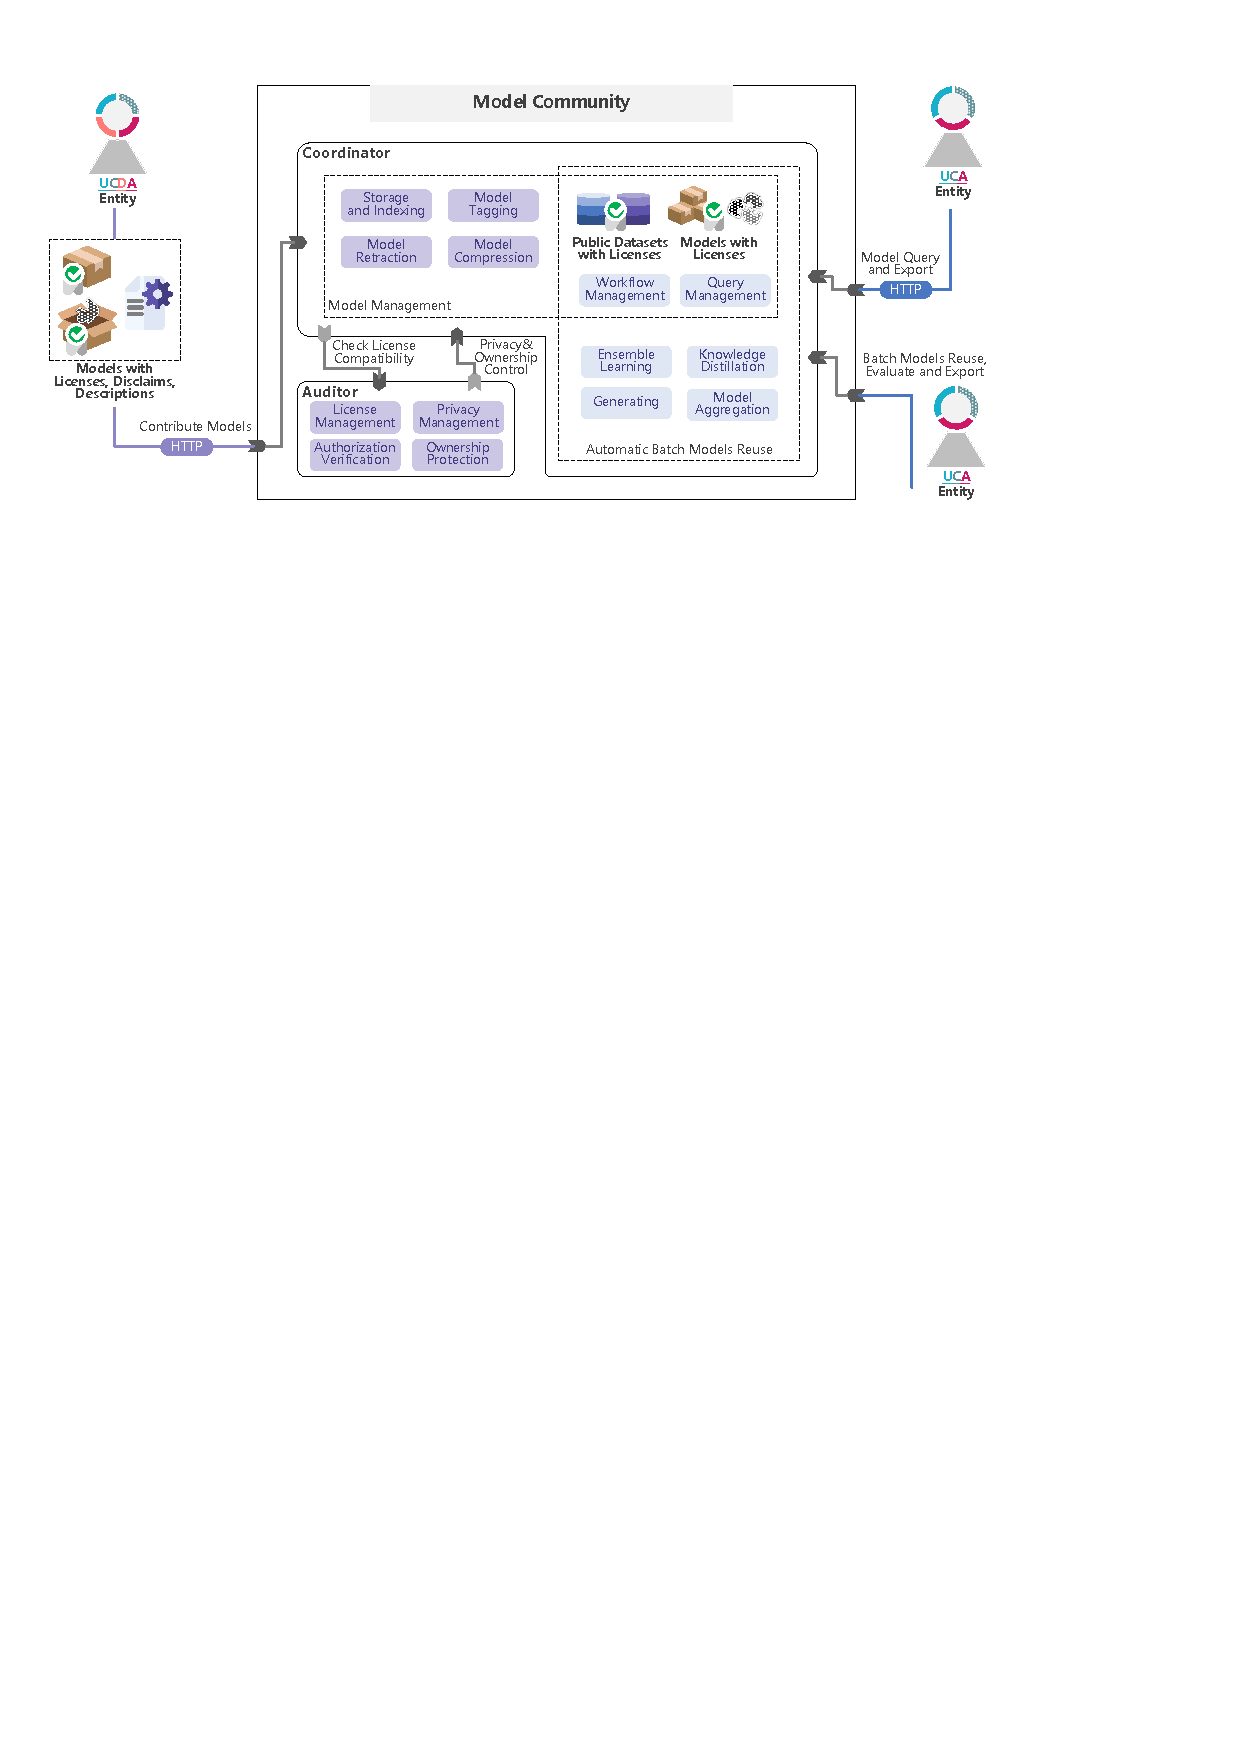
\includegraphics[width=\linewidth]{fig/query_frame.pdf}
  \caption{An overview of query-based FL systems. (U: model User, C: Coordinator, D: Data owner, A: Auditor)}
  \Description{}
  \label{fig:query}
\end{figure}

\subsection{How to Query Model}


HOw

\begin{table}[t]
  \caption{Summary of existing deep learning model repositories.}
  \label{table:repository}
  \footnotesize
  \begin{tabular}{|l|c|c|c|c|c|c|c|c|}
  \hline
  & \multicolumn{1}{l|}{DS Name} & \multicolumn{1}{l|}{Model Architecture} & \multicolumn{1}{l|}{Modality/Task} & \multicolumn{1}{l|}{Tag} & \multicolumn{1}{l|}{License} & \multicolumn{1}{l|}{Input-Output} & \multicolumn{1}{l|}{Batch Export} & \multicolumn{1}{l|}{\# of Models}\\ \hline
  Hugging Face\tablefootnote{https://huggingface.co}
  & \checkmark & \checkmark & \checkmark & \checkmark & \checkmark & \textbf{!} & \ding{55} & 133,641 \\ \hline
  Model Zoo\tablefootnote{https://modelzoo.co/} & \checkmark & \checkmark & \checkmark & \checkmark & \ding{55} & \ding{55} & \ding{55} & 3,426 \\ \hline
  OpenVINO\tablefootnote{https://docs.openvino.ai/latest/model\_zoo.html} & \textbf{!} & \checkmark & \checkmark & \ding{55} & \textbf{!} & \textbf{!} & \checkmark & 278 \\ \hline
  Tensorflow Hub\tablefootnote{https://tfhub.dev/}& \checkmark & \checkmark & \checkmark & \checkmark & \textbf{!} & \textbf{!} & \ding{55} & 1,356 \\ \hline
  Pytorch Hub\tablefootnote{https://pytorch.org/hub/} & \textbf{!} & \checkmark & \ding{55} & \ding{55} & \ding{55} & \textbf{!} & \ding{55} & 49 \\ \hline
  NVIDIA NGC\tablefootnote{https://catalog.ngc.nvidia.com/models} & \textbf{!} & \checkmark & \checkmark & \checkmark & \textbf{!} & \textbf{!} & \ding{55} & 527 \\ \hline
  \end{tabular}
\end{table}

We descibe the structure of 

The properties are: (1) Model Agnostic; (2) Contactless; (3) Community-powered

Model type?

Model heterogeneity?

Black box, White box, Mix?

With val?

Horizontal or Vertical?

\begin{table}[t]
    \centering
    \scriptsize
    \caption{Licenses for ML models available on Hugging Face with a focus on their rights, scopes and restrictions, grouped by free software licenses, AI model licenses, free content or database licenses in descending order of number of models (GPL, BSD, LGPL, CC licenses with unspecified versions are excluded, the similar revisions are merged)}
    \label{tab:licenses}
    \begin{tabular}{r||ccc|ccc|cccc|c|p{3.5cm}}
    \toprule
    Licenses
    & \multicolumn{1}{P{90}{2.0cm}}{Modify / Merge} &
      \multicolumn{1}{P{90}{2.0cm}}{Redistribution} &
      \multicolumn{1}{P{90}{2.0cm}}{Sublicensing} & 
      \multicolumn{1}{P{90}{2.0cm}}{Commercial Use} & 
      \multicolumn{1}{P{90}{2.0cm}}{Patent Use} & 
      \multicolumn{1}{P{90}{2.0cm}}{Trademark Use} &
      \multicolumn{1}{P{90}{2.0cm}}{State Changes} &
      \multicolumn{1}{P{90}{2.0cm}}{Disclose Source} &
      \multicolumn{1}{P{90}{2.0cm}}{Behavioral-use Restrictions} &
      \multicolumn{1}{P{90}{2.0cm}}{License/Disclaim Preservation} &
      \multicolumn{1}{P{90}{2.0cm}}{\# of Models} &
      \multicolumn{1}{c}{Examples / Remarks}    \\
    \midrule
    Apache-2.0 & \checkmark & \checkmark & \checkmark & \checkmark & \checkmark & \ding{55} & \checkmark & \ding{55} & \ding{55} & \checkmark & 23,519 & BERT \\
    MIT &  \checkmark & \checkmark & \checkmark & \checkmark & \textbf{!} & \textbf{!} & \ding{55} & \ding{55} & \ding{55} & \checkmark & 9,605 & GPT2 \\
    AFL-3.0 & \checkmark & \checkmark & \checkmark & \checkmark & \checkmark & \ding{55} & \checkmark & \ding{55} & \ding{55} & \checkmark & 1,561 & Italian-Legal-BERT \\
    GPL-3.0 & \checkmark & \checkmark & \ding{55} & \checkmark & \checkmark & \ding{55} & \checkmark & \checkmark & \ding{55} & \checkmark & 404 & CKIP BERT Chinese \\
    Artistic-2.0 & \checkmark & \checkmark & \checkmark & \checkmark & \checkmark & \ding{55} & \checkmark & \ding{55} & \ding{55} & \checkmark & 331 & Include original source \\
    BSD-3-Clause\&-Clear & \checkmark & \checkmark & \checkmark & \checkmark & \textbf{!} & \textbf{!} & \ding{55} & \ding{55} & \ding{55} & \checkmark & 209 & CodeGen / a MIT-style license \\
    WTFPL-2.0 & \checkmark & \checkmark & \textbf{!} & \checkmark & \textbf{!} & \textbf{!} & \ding{55} & \ding{55} & \ding{55} & \ding{55} & 131 & A MIT-style permissive license  \\
    AGPL-3.0 & \checkmark & \checkmark & \ding{55} & \checkmark & \checkmark & \ding{55} & \checkmark & \checkmark & \ding{55} & \checkmark & 96 & Distributed under AGPL only  \\
    Unlicense & \checkmark & \checkmark & \textbf{!} & \checkmark & \textbf{!} & \textbf{!} & \ding{55} & \ding{55} & \ding{55} & \ding{55} & 90 & A MIT-style permissive license  \\
    %GPL & 1 & 2 & 3 & 4 & 5 & 6 & 7 & 8 & 9 & 10 & 63 &  \\
    BSL-1.0 & \checkmark & \checkmark & \checkmark & \checkmark & \textbf{!} & \textbf{!} & \ding{55} & \ding{55} & \ding{55} & \checkmark & 60 & A MIT-style permissive license \\
    %BSD & 1 & 2 & 3 & 4 & 5 & 6 & 7 & 8 & 9 & 10 & 43 &  \\
    GPL-2.0 & \checkmark & \checkmark & \ding{55} & \checkmark & \textbf{!} & \textbf{!} & \checkmark & \checkmark & \ding{55} & \checkmark & 34 & Not compatible with GPL-3.0  \\
    BSD-2-Clause & \checkmark & \checkmark & \checkmark & \checkmark & \textbf{!} & \textbf{!} & \ding{55} & \ding{55} & \ding{55} & \checkmark & 34 & A MIT-style permissive license  \\
    LGPL-2.1\&3.0 & \checkmark & \checkmark & \ding{55} & \checkmark & \textbf{!} & \textbf{!} & \checkmark & \checkmark & \ding{55} & \checkmark & 25 & For software libraries  \\
    OSL-3.0 & \checkmark & \checkmark & \checkmark & \checkmark & \checkmark & \ding{55} & \checkmark & \checkmark & \ding{55} & \checkmark & 22 & Linking is not derivative work \\
    %BSD-3-Clause-Clear & 1 & 2 & 3 & 4 & 5 & 6 & 7 & 8 & 9 & 10 & 14 &  \\
    %LGPL & 1 & 2 & 3 & 4 & 5 & 6 & 7 & 8 & 9 & 10 & 12 &  \\
    ECL-2.0 & \checkmark & \checkmark & \checkmark & \checkmark & \checkmark & \ding{55} & \checkmark & \ding{55} & \ding{55} & \checkmark & 12 & For education communities \\
    MPL-2.0 & \checkmark & \checkmark & \checkmark & \checkmark & \checkmark & \ding{55} & \checkmark & \checkmark & \ding{55} & \checkmark & 9 & State changes under MPL only  \\
    ISC & \checkmark & \checkmark & \textbf{!} & \checkmark & \textbf{!} & \textbf{!} & \ding{55} & \ding{55} & \ding{55} & \checkmark & 8 & MIT-style license w/o sublicense \\ % Permission to distribute this software for any purpose
    Zlib & \checkmark & \checkmark & \textbf{!} & \checkmark & \textbf{!} & \textbf{!} & \ding{55} & \ding{55} & \ding{55} & \checkmark & 8 & Rename if modified \\
    Ms-PL & \checkmark & \checkmark & \checkmark & \checkmark & \checkmark & \ding{55} & \ding{55} & \ding{55} & \ding{55} & \checkmark & 7 & MIT-style with patent granted \\
    EPL-1.0\&2.0 & \checkmark & \checkmark & \checkmark & \checkmark & \checkmark & \textbf{!} & \ding{55} & \checkmark & \ding{55} & \checkmark & 6 & Can link proprietary license code \\
    NCSA & \checkmark & \checkmark & \checkmark & \checkmark & \textbf{!} & \ding{55} & \ding{55} & \ding{55} & \ding{55} & \checkmark & 4 & Include full text of license \\
    PostgreSQL & \checkmark & \checkmark & \textbf{!} & \checkmark & \textbf{!} & \textbf{!} & \ding{55} & \ding{55} & \ding{55} & \checkmark & 2 & A MIT-style license \\
    OFL-1.1 & \checkmark & \checkmark & \ding{55} & \checkmark & \textbf{!} & \textbf{!} & \ding{55} & \ding{55} & \ding{55} & \checkmark & 2 & For font software \\
    %EPL-1.0 & 1 & 2 & 3 & 4 & 5 & 6 & 7 & 8 & 9 & 10 & 2 &  \\
    EUPL-1.1 & \checkmark & \checkmark & \checkmark & \checkmark & \checkmark & \ding{55} & \checkmark & \checkmark & \ding{55} & \checkmark & 1 & License of EU covers SaaS \\
    %LGPL-2.1 & 1 & 2 & 3 & 4 & 5 & 6 & 7 & 8 & 9 & 10 & 1 &  \\
    LPPL-1.3c & \checkmark & \checkmark & \checkmark & \checkmark & \textbf{!} & \ding{55} & \checkmark & \checkmark & \ding{55} & \checkmark & 1 & Covering  stewardship transfer \\
    
    \hline
    %\textbf{Model Licenses $\downarrow$} & \multicolumn{12}{l}{} \\
    \hline
    
    CreativeML-OpenRAIL-M & \checkmark & \checkmark & \checkmark & \checkmark & \checkmark & \ding{55} & \checkmark & \ding{55} & \checkmark & \checkmark & 3,590 & Stable Diffusions v1 \\
    OpenRAIL &  \multicolumn{10}{l|}{>Responsible AI License template, w/o full text} & 2,393 & ControlNet  \\
    BigScience-BLOOM-RAIL-1.0 & \checkmark & \checkmark & \checkmark & \checkmark & \checkmark & \ding{55} & \checkmark & \ding{55} & \checkmark & \checkmark & 196 & BLOOM \\
    BigScience-OpenRAIL-M & \multicolumn{10}{l|}{>Same as BigScience-BLOOM-RAIL-1.0} & 155 & (A General Version of 1.0) \\
    OpenRAIL++ & \multicolumn{10}{l|}{>Same as CreativeML-OpenRAIL-M} & 72 & Stable Diffusion v2 \\
    OPT-175B & \checkmark & \ding{55} & \ding{55} & \ding{55} & \ding{55} & \ding{55} & \ding{55} & \ding{55} & \checkmark & \checkmark & $\approx66$ & OPT-175B LLM \\
    SEER &  \multicolumn{10}{l|}{>Same as OPT-175B, ban on reverse-engineer} & / & SEER Vision Model \\
    
    \hline
    \hline

    CC-BY-4.0\&3.0\&2.5\&2.0 & \checkmark & \checkmark & \ding{55} & \checkmark & \ding{55} & \ding{55} & \checkmark & \ding{55} & \ding{55} & \checkmark & 1,740 & RoBERTa \\
    CC-BY-SA-4.0\&3.0 &  \checkmark & \checkmark & \ding{55} & \checkmark & \ding{55} & \ding{55} & \checkmark & \checkmark & \ding{55} & \checkmark & 590 & LEGAL-BERT \\
    CC-BY-NC-SA-4.0\&3.0 & \checkmark & \checkmark & \ding{55} & \ding{55} & \ding{55} & \ding{55} & \checkmark & \checkmark & \ding{55} & \checkmark & 556 & LayoutLMv3 \\
    CC-BY-NC-4.0\&3.0\&2.0 & \checkmark & \checkmark & \ding{55} & \ding{55} & \ding{55} & \ding{55} & \checkmark & \ding{55} & \ding{55} & \checkmark & 499 & GALACTICA \\
    CC0-1.0 & \checkmark & \checkmark & \ding{55} & \checkmark & \ding{55} & \ding{55} & \ding{55} & \ding{55} & \ding{55} & \ding{55} & 165 & BlueBERT \\
    CC-BY-NC-ND-4.0\&3.0 & \checkmark & \ding{55} & \ding{55} & \ding{55} & \ding{55} & \ding{55} & \ding{55} & \ding{55} & \ding{55} & \checkmark & 21 & NonCommercial, NoDerivatives \\
    PDDL & \checkmark & \checkmark & \ding{55} & \checkmark & \ding{55} & \ding{55} & \ding{55} & \ding{55} & \ding{55} & \ding{55} & 16 & Database-specific license \\
    C-UDA & \checkmark & \checkmark & \checkmark & \ding{55} & \textbf{!} & \textbf{!} & \ding{55} & \ding{55} & \checkmark & \checkmark & 13 & Data for computational use only \\
    LGPL-LR & \checkmark & \checkmark & \ding{55} & \checkmark & \textbf{!} & \textbf{!} & \checkmark & \checkmark & \ding{55} & \checkmark & 12 & LGPL for linguistic resources \\ %如果仅仅发布embedding模型,那么属于属于“使用语言资源的作品”,如果包含了语言资源或者加密后的资源,那么属于“使用语言资源的衍生物”,包含在此license范围
    GFDL &  \multicolumn{10}{l|}{>Same as GPL, a free document license} & 12 & txtai-wikipedia \\
    CC-BY-ND-4.0 & \checkmark & \ding{55} & \ding{55} & \checkmark & \ding{55} & \ding{55} & \checkmark & \ding{55} & \ding{55} & \checkmark & 11 & Disallow making derivatives \\
    ODC-By & \checkmark & \checkmark & \ding{55} & \checkmark & \ding{55} & \ding{55} & \ding{55} & \ding{55} & \ding{55} & \checkmark & 7 & Database license w/o sublicense \\
    ODbL & \checkmark & \checkmark & \ding{55} & \checkmark & \ding{55} & \ding{55} & \checkmark & \checkmark & \ding{55} & \checkmark & 6 & Automatic relicensing \\
    \bottomrule
    \end{tabular}
  \end{table}
  


Query syntax: Table.~\ref{table:repository}, data description, workflow metadata/history of ML pipeline (Scientific workflow management), model performance and profile (task-specific), software dependency,
model use mode

CreativeML Open RAIL-M:
we added use-based restrictions not permitting the use of the Model in very specific scenarios, in order for the licensor to be able to enforce the license in case potential misuses of the Model may occur.